% Chapter 3 standalone build in Texas A&M (OGAPS) thesis format with IEEE citations.
% Build: pdflatex main_ch3 && bibtex main_ch3 && pdflatex main_ch3 && pdflatex main_ch3
\documentclass[12pt,letterpaper]{report}

\usepackage[T1]{fontenc}
\usepackage[utf8]{inputenc}
\usepackage{newtxtext,newtxmath}          % Times-style text and math
\usepackage[margin=1in]{geometry}         % TAMU: 1-inch margins
\usepackage{setspace}
\doublespacing                            % TAMU: double-spaced body text
\usepackage{graphicx}
\usepackage{amsmath}
\graphicspath{{../../tpec2027/figures/}}
\usepackage{booktabs,tabularx,array}
\usepackage{cite}                         % IEEE-style compressed numeric citations [1]-[4]
\usepackage[labelsep=period,font={singlespacing}]{caption}
\usepackage{titlesec}
\usepackage[hidelinks]{hyperref}

% --- TAMU-style headings: centered, all-caps chapter title; numbered sections
\titleformat{\chapter}[block]{\normalfont\bfseries\centering}{\thechapter.}{0.5em}{\MakeUppercase}
\titleformat{name=\chapter,numberless}[block]{\normalfont\bfseries\centering}{}{0pt}{\MakeUppercase}
\titlespacing*{\chapter}{0pt}{0pt}{12pt}
\titleformat{\section}{\normalfont\bfseries}{\thesection}{0.75em}{}
\titlespacing*{\section}{0pt}{12pt}{0pt}
\renewcommand{\bibname}{References}

% Float pages: start floats at the top of the page
\makeatletter
\setlength{\@fptop}{0pt}
\setlength{\@fpsep}{12pt}
\makeatother

% TAMU: figure/table numbering by chapter (Figure 2.1, Table 2.1)
\renewcommand{\figurename}{Figure}

\begin{document}
\setcounter{chapter}{2}   % this file is Chapter 3 of the dissertation
% Chapter 3 of the dissertation: the EEF concept, the planning model, the scenarios and the national grid context.
% Build with main_ch3.tex. Numbers come from tpec2027/results/*.csv (scripts listed in Section 3.12).
\chapter{External Energy Flexibility: Concept, Planning Model and Scenarios}\label{ch:model}

\section{Introduction}\label{sec:3-1}

Chapter~2 found no framework in which an inflexible AI data center uses the flexibility of \emph{other} loads on the grid to obtain hourly clean supply. This chapter proposes that framework, External Energy Flexibility (EEF), and answers the first research question: how EEF can be formalized, and how it compares with direct grid supply (GRID), annual matching (AM) and photovoltaics with batteries (RE+BESS) on reliability, cost and sustainability.

The chapter has four parts. Sections~\ref{sec:3-2}--\ref{sec:3-3} define the concept and the four supply configurations. Sections~\ref{sec:3-4}--\ref{sec:3-7} state the data, the linear programs, the cost model and the sweep that derives the displacement target and the range of data-center sizes instead of assuming them. Sections~\ref{sec:3-8}--\ref{sec:3-10} report the results at the recommended 90\% target and the scenarios along both curves: displacement from 42\% to 100\%, and size from 0.1~MW to 6~GW. Section~\ref{sec:3-11} sets those scenarios against the Saudi grid, whose capacity is about 90~GW and whose peak is growing by about 3~GW a year. Section~\ref{sec:3-12} lists the code, and Sections~\ref{sec:3-13}--\ref{sec:3-14} state the limitations and summarize.

\section{The EEF Concept}\label{sec:3-2}

\subsection{Actors and Flows}

Figure~\ref{fig:3-arch} shows the arrangement. Four rules define it.

\begin{enumerate}
\item \textbf{The data center stays on the grid.} It buys 100\% of its consumption from the grid at the regulated tariff in every hour, so its reliability is that of the grid.
\item \textbf{The data center uses none of the PV output.} A PV plant whose annual output equals the data center's annual consumption injects all its energy into the grid and sells it to the single buyer (SPPC) under a power purchase agreement.
\item \textbf{Existing flexible loads absorb all of the PV output.} Through contracts with the grid and an aggregator, loads already connected anywhere on the national grid (desalination, district cooling with thermal storage, water pumping and industry) raise their consumption while the PV plant generates.
\item \textbf{The same loads step back by the data center's load.} In return, every hour they reduce their consumption below their metered baseline by the data center's consumption. The grid supply they free is credited to the data center. Each load is energy-neutral within its shifting window: it moves consumption, it does not add it.
\end{enumerate}

Because absorption and reduction overlap in daylight, the loads' physical deviation from baseline is the net of the two. It is an increase equal to the PV output minus the data center's load around midday, and a decrease equal to the data center's load at night. For a 100-MW data center at noon with 350~MW of PV output, the loads absorb 350~MW and step back 100~MW, a net increase of 250~MW; at 02:00 they step back 100~MW. The term \emph{displacement} $X$ denotes the share of the data center's annual consumption whose grid supply is freed hour by hour in this way. It is the quantity that the literature calls hourly matching or the carbon-free-energy (CFE) score.

\begin{figure}[!htbp]
\centering
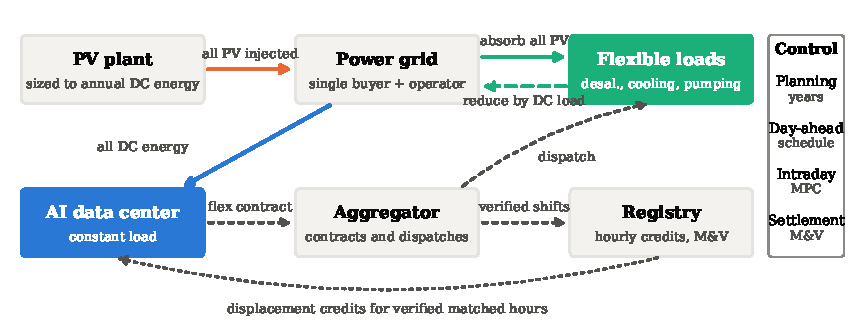
\includegraphics[width=\textwidth]{fig1_architecture.pdf}
\caption{EEF architecture. Solid arrows: energy; dashed: contracts, dispatch and verification; dotted: credits. The control layers act only on the external loads, never on the data center.}
\label{fig:3-arch}
\end{figure}

\subsection{Hourly Accounting Rule}

In each hour $t$, the data center is credited with the grid supply freed for it by the flexible loads, up to its consumption, only if two conditions hold. First, the same loads absorbed an equal amount of PV output within the same window. Second, their net deviations are verified against their baselines with interval metering. The PV output itself is credited to the loads that absorb it, never to the data center. Credits are recorded as hourly certificates in a registry \cite{r51}, which prevents double counting with other flexibility services.

\subsection{Control Layers}

EEF is controlled in four layers, all acting on the flexible loads and none on the data center:
\begin{itemize}
\item \emph{planning} (years): sizes the PV plant and the contracted flexible power and energy; this chapter;
\item \emph{day-ahead} scheduling (24~h): forecasts PV and load, computes the hourly gap and dispatches the cheapest flexibility first, subject to the system operator's network checks;
\item \emph{intraday} model-predictive correction (minutes): re-dispatches the loads as forecasts change; residual error is absorbed by the grid and counted as unmatched;
\item \emph{settlement} (monthly): verifies shifts against baselines, issues credits and pays the loads.
\end{itemize}
Because control never acts on the data center, the worst case of EEF is annual matching with unchanged reliability. The day-ahead and intraday layers are the subject of Chapter~4.

\section{Supply Configurations and Metrics}\label{sec:3-3}

Table~\ref{tab:3-configs} defines the four configurations. All four buy the data center's entire consumption from the grid and share the same PV plant where they have one, so their differences are the cost of hourly matching, the emissions it avoids and the load the data center leaves on the grid.

\begin{table}[!htbp]
\centering
\caption{The four supply configurations compared.}
\label{tab:3-configs}
\small
\renewcommand{\arraystretch}{1.2}
\begin{tabularx}{\textwidth}{>{\raggedright\arraybackslash}p{2.2cm}>{\raggedright\arraybackslash}X>{\raggedright\arraybackslash}p{4.4cm}}
\toprule
\textbf{Label} & \textbf{Configuration} & \textbf{Today's equivalent in Saudi Arabia} \\
\midrule
GRID & Direct grid supply, no clean procurement & Today's default \\
AM & PV equal to annual use, injected and sold; annual certificates & Today's ``green'' claim (I-RECs) \\
RE+BESS & Same PV plus a battery charged from PV output in excess of the data center's same-hour load & The storage route \\
EEF & Same PV plus contracted external flexible loads & This work \\
\bottomrule
\end{tabularx}
\end{table}

The three pillars are measured as follows.
\begin{itemize}
\item \textbf{Reliability:} the share of the data center's load served. It is 100\% in all four configurations because the data center is always supplied by the grid. The impact on the grid is reported separately as the load the data center leaves on the grid on summer evenings (June--September, 18:00--02:00), the hours that drive reinforcement.
\item \textbf{Sustainability:} displacement $X$ and hourly-accounted emissions at the average grid factor of 0.568~tCO$_2$/MWh \cite{kfupmghg}.
\item \textbf{Cost:} the annual cost of hourly matching, the break-even flexibility price against storage, and a unit cost that adds grid reinforcement and carbon (Section~\ref{sec:3-6}).
\end{itemize}

\section{Data and Parameters}\label{sec:3-4}

The base case is a constant 100-MW AI data center in Riyadh (24.71$^\circ$N, 46.68$^\circ$E) that consumes 876~GWh/yr. Hourly PV output for 2020 comes from PVGIS-SARAH3 for fixed, optimally tilted crystalline-silicon modules with 14\% system losses \cite{pvgis}. The capacity factor is 20.96\%, so a 477-MWp plant matches the annual consumption. The second site is NEOM--Oxagon on the Red Sea coast (27.40$^\circ$N, 35.60$^\circ$E; capacity factor 21.37\%). Table~\ref{tab:3-params} lists the parameters. Prices are converted at 3.75~SAR per US\$.

\begin{table}[!htbp]
\centering
\caption{Case-study parameters.}
\label{tab:3-params}
\small
\renewcommand{\arraystretch}{1.15}
\begin{tabularx}{\textwidth}{>{\raggedright\arraybackslash}X>{\raggedright\arraybackslash}p{5.6cm}}
\toprule
\textbf{Parameter} & \textbf{Value} \\
\midrule
Data-center load & 100~MW, constant (base); 0.1~MW--6~GW in the scenarios \\
PV plant (annual matching) & 477~MWp; capacity factor 20.96\% \cite{pvgis} \\
PV selling price & US\$13.6/MWh, equal to its cost (NREP benchmark; assumption) \\
Grid tariff (cloud computing) & 0.18~SAR/kWh = US\$48/MWh \cite{kapsarcdc} \\
Battery capital cost, 2030, 4-h & US\$124/207/338 per kWh, low/mid/high \cite{nrelbess2025} \\
Battery round-trip efficiency & 90\% \\
Discount rate; battery life; fixed O\&M; horizon & 8\%; 15~yr; 2.5\%/yr; 25~yr \\
Flexibility shifting efficiency $\eta$ & 0.95 (0.85--1.0) \\
Shifting duration $D$ & 8~h (4 and 12~h tested) \\
Flexibility price $\pi$ & US\$50 (25--75) per MWh shifted (assumption) \\
Grid reinforcement $R$ & US\$125/kW-yr (100--150; assumption) \\
Carbon price $\kappa$ & US\$50/t (assumption) \\
EEF contract overhead $F$ & US\$0.25~M/yr per contract (0.1--0.5; assumption) \\
Grid emission factor (average) & 0.568~tCO$_2$/MWh \cite{kfupmghg} \\
National flexible-load pool & unlimited; 29.9~GW; 7.1~GW \cite{r23} \\
\bottomrule
\end{tabularx}
\end{table}

\section{Planning Model}\label{sec:3-5}

\subsection{Hourly Matching}

Let $L_t$ be the data-center load and $P_t$ the PV output in hour $t\in\mathcal{T}$, $|\mathcal{T}|=8760$. Netting the loads' absorption of PV and their reduction for the data center in each hour gives a net increase bounded by the surplus $s_t=[P_t-L_t]^+$ or a net decrease bounded by the deficit $g_t=[L_t-P_t]^+$. Displacement is
\begin{equation}
X=\frac{\sum_t \min(L_t,P_t)+\sum_t m_t}{\sum_t L_t},
\label{eq:3-cfe}
\end{equation}
where $m_t\le g_t$ is the deficit covered by credited flexibility ($m_t=d_t$ for EEF) or by battery discharge ($m_t=b_t$). The first term is the part of the loads' absorption that is offset in the same hour by their reduction for the data center. It is not consumption of PV by the data center. Under AM, $m_t=0$ and $X=40.4\%$ in Riyadh.

\subsection{EEF Linear Program}

The flexible portfolio is represented by one aggregated class with contracted power $P^F$, shiftable energy $D\,P^F$ and shifting efficiency $\eta$. The decision variables are the net up-shift $u_t$, the net down-shift $d_t$ and the shifted energy $S_t$:
\begin{align}
S_t &= (1-\delta_t)\,S_{t-1}+\eta\,u_t-d_t, \label{eq:3-state}\\
0\le u_t &\le \min(P^F,s_t),\qquad 0\le d_t\le\min(P^F,g_t), \label{eq:3-bounds}\\
0\le S_t &\le D\,P^F,\qquad S_t=0\quad \forall t\in\mathcal{E}. \label{eq:3-energy}
\end{align}
Here $\delta_t=1$ in the first hour of each window and $\mathcal{E}$ is the set of window-end hours, so every window is energy-neutral. The base window runs 24~h from 06:00; windows from 09:00 and week-long windows are tested in the sweep. Two programs use these constraints:
\begin{align}
\text{min-capacity:}\quad &\min\ P^F\quad\text{s.t. (\ref{eq:3-state})--(\ref{eq:3-energy})},\ \ \textstyle\sum_t d_t\ \ge\ X\sum_t L_t-\sum_t\min(L_t,P_t), \label{eq:3-min}\\
\text{max-displacement:}\quad &\max\ \textstyle\sum_t d_t\quad\text{s.t. (\ref{eq:3-state})--(\ref{eq:3-energy}) for a given } P^F. \label{eq:3-max}
\end{align}
A tie-break cost of $10^{-6}$ per MWh on $u_t$ in (\ref{eq:3-min}) avoids unnecessary shifting.

\subsection{Battery Linear Program}

A battery of energy capacity $E$ charges $c_t\le s_t$ and discharges $b_t\le g_t$, with state of charge
\begin{equation}
Q_t=Q_{t-1}+\eta_c\,c_t-b_t/\eta_d,\qquad 0\le Q_t\le E,\qquad Q_0=Q_{|\mathcal{T}|},
\end{equation}
where $\eta_c=\eta_d=\sqrt{0.9}$. The program minimizes $E$ subject to $\sum_t b_t\ge X\sum_tL_t-\sum_t\min(L_t,P_t)$. Its annual cost is $C^B=c_E E\,(\mathrm{CRF}+\phi)$ with capital cost $c_E$, capital recovery factor CRF (8\%, 15~yr) and fixed O\&M share $\phi$. Only energy capacity is charged, which favors storage.

\subsection{Break-Even Flexibility Price}

Because EEF and RE+BESS share the same PV plant and grid supply, EEF is cheaper than storage at target $X$ when the payment per MWh shifted is below
\begin{equation}
\pi^\ast(X)=C^B(X)\,\big/\,\textstyle\sum_t d_t(X).
\label{eq:3-breakeven}
\end{equation}

\subsection{Solution Method}

All programs are linear: the state, bounds and energy-neutrality constraints are linear in the variables, and there are no fixed costs or on/off decisions at the planning level. A linear program has a global optimum, which a solver finds exactly, so every result is reproducible and comparable across scenarios. The programs are solved with HiGHS \cite{highs} through the \texttt{linprog} function of SciPy in Python \cite{scipy}, with the constraint matrices built as sparse matrices. The min-capacity program (\ref{eq:3-min}) has $3\cdot8760+1=26{,}281$ variables and $35{,}041$ constraints ($8{,}760$ equalities and $26{,}281$ inequalities); the battery program has $26{,}281$ variables and $17{,}521$ constraints. Each solves in 0.5--1.3~s (Table~\ref{tab:3-scaling}). Mixed-integer programming would be needed only if discrete unit sizes mattered, and stochastic or robust programming only for operation under uncertainty (Chapter~4).

\section{Cost Model and Decision Rule}\label{sec:3-6}

All configurations pay the same tariff for all of the data center's consumption, and PV is sold at its cost, so the tariff and the PV plant cancel. Configuration $j$ is therefore compared by its cost per MWh of data-center consumption \emph{above} the tariff,
\begin{equation}
c_j(X,S)=\frac{C^M_j(X)}{E}+\frac{R\,(1-\rho_j)}{8.76}+\kappa\,e\,(1-X_j)+\frac{F_j}{8760\,S},
\label{eq:3-unitcost}
\end{equation}
where:
\begin{itemize}
\item $C^M_j$ is the annual matching cost: zero for GRID and AM, $C^B$ for RE+BESS and $\pi\sum_t d_t$ for EEF;
\item $E$ is the annual consumption in MWh;
\item $R$ is the grid-reinforcement cost (US\$/kW-yr), charged on the share $1-\rho_j$ of the data center's summer-evening load that is not freed;
\item $\kappa$ is the carbon price, $e$ the emission factor and $X_j$ the displacement;
\item $F_j$ is a fixed annual EEF contract overhead (metering, measurement and verification, registry, aggregator administration), spread over the data-center size $S$ in MW.
\end{itemize}

With the base values, GRID costs US\$42.7/MWh (US\$14.3 of reinforcement and US\$28.4 of carbon) and AM US\$31.2/MWh. EEF \emph{works} at $(X,S)$ when two conditions hold: it has the lowest $c_j$ of the four configurations, and it frees at least 90\% of the data center's summer-evening load. The second condition ensures that EEF relieves the grid where reinforcement is decided, not only on an annual average.

\section{Deriving the Target and the Size Range}\label{sec:3-7}

\subsection{The Sweep}

The target and the size range are derived rather than assumed. For each target $X$ from 42\% to 99.9\%, the procedure is:
\begin{enumerate}
\item solve the min-capacity EEF program and the battery program for six designs: PV multiples $k\in\{1,1.25,1.5,2,3\}$ of the annual-matching plant, windows from 06:00 ($k=1$) or 09:00, and a week-long window ($k=2$);
\item keep the designs allowed at $X$: daily windows with $k\le\max(1.25,k_{\min}(X))$, where $k_{\min}(X)$ is the smallest multiple that reaches $X$; week-long windows only where no daily design reaches $X$;
\item choose for EEF and for the battery, separately, the allowed design with the lowest cost (\ref{eq:3-unitcost});
\item record the flexible power, the battery energy, the energy shifted, and the share of summer evenings freed.
\end{enumerate}
The sweep solves 66 linear programs for Riyadh and 70 for NEOM (one EEF and one battery program per target and design, plus the maximum displacement of each design).

\subsection{Why EEF Stops Short of 100\%}

Even with unlimited flexibility, the base design reaches at most 91.2\%. The gap from 100\% decomposes into three parts: the shifting loss ($\eta=0.95$) caps an annual window at 97.0\%; daily windows lose days on which PV output cannot cover the night (94.6\%); and the order of hours within each window loses the early-morning deficit before PV starts (91.2\%). A window from 09:00 lets the morning draw on the previous day's PV and raises the ceiling to 93.4\% with $k=1$ and 98.1\% with $k=1.25$. Larger plants raise it to 98.7\% ($k=1.5$), 99.2\% ($k=2$) and 99.6\% ($k=3$), and loads that shift across a week reach about 99.9\%. The last 0.1\% is the first hours of the year, before any PV, a boundary effect of the one-year horizon. One hundred percent is therefore out of reach.

\subsection{Why Size Does Not Change the Physics}\label{sec:3-7-3}

Scaling the load and the PV plant by a factor $\lambda$ scales every feasible solution of (\ref{eq:3-state})--(\ref{eq:3-max}) by $\lambda$: if $(u,d,S,P^F)$ is feasible for $(L,P)$, then $(\lambda u,\lambda d,\lambda S,\lambda P^F)$ is feasible for $(\lambda L,\lambda P)$ with the same displacement, and the optimum scales the same way because the objective is linear. The same holds for the battery program. Table~\ref{tab:3-scaling} confirms this numerically by re-solving the 90\% target at 10, 100 and 1,000~MW: every result per MW is identical. Size therefore enters the comparison only through the contract overhead $F$ and the national flexible-load pool.

\begin{table}[!htbp]
\centering
\caption{Numerical check of linear scaling at the 90\% target (Riyadh, PV $=$ annual use, window from 06:00, $D=8$~h).}
\label{tab:3-scaling}
\small
\begin{tabular}{@{}rcccccc@{}}
\toprule
\textbf{Data center} & \textbf{PV} & \textbf{Flexible power} & \textbf{Battery} & \textbf{Shifted} & \multicolumn{2}{c}{\textbf{Solve time (s)}} \\
(MW) & (MWp/MW) & (MW/MW) & (MWh/MW) & (\% of load) & EEF & Battery \\
\midrule
10 & 4.7706 & 2.0288 & 13.195 & 49.57 & 1.24 & 0.52 \\
100 & 4.7706 & 2.0288 & 13.195 & 49.57 & 0.96 & 0.53 \\
1,000 & 4.7706 & 2.0288 & 13.195 & 49.57 & 0.91 & 0.52 \\
\bottomrule
\end{tabular}
\end{table}

With the per-MW costs fixed, (\ref{eq:3-unitcost}) gives EEF a cost that falls as $F/(8760\,S)$. EEF overtakes a competitor $j$ at the size
\begin{equation}
S^\ast_j=\frac{F}{8760\,\Delta_j},
\label{eq:3-threshold}
\end{equation}
where $\Delta_j$ is EEF's saving per MWh against $j$ before the overhead. At 90\%, $\Delta=\$3.48$/MWh against AM, the cheapest alternative, and \$17.7/MWh against the battery, so $S^\ast=8.2$~MW and 1.6~MW. Table~\ref{tab:3-overhead} shows how these thresholds move with the overhead. The lower end of the size range is therefore a matter of contract cost, and smaller sites can share one contract.

\begin{table}[!htbp]
\centering
\caption{Smallest data center for which EEF wins at 90\%, by contract overhead (Riyadh).}
\label{tab:3-overhead}
\small
\begin{tabular}{@{}ccc@{}}
\toprule
\textbf{Overhead $F$ (US\$~M/yr)} & \textbf{Cheapest of all four from} & \textbf{Cheaper than the battery from} \\
\midrule
0.10 & 3.3~MW & 0.6~MW \\
0.25 (base) & 8.2~MW & 1.6~MW \\
0.50 & 16.4~MW & 3.2~MW \\
\bottomrule
\end{tabular}
\end{table}

\subsection{The Resulting Target and Size Range}

Figure~\ref{fig:3-verdict} shows the two curves for Riyadh and NEOM. Along the displacement curve, EEF is the cheapest option from 45\% upward, but below 85\% it leaves part of the summer-evening load on the grid (83\% freed at 80\%). EEF therefore works for targets of 85--99.5\%. Within this range, 90\% is the recommended target for three reasons:
\begin{enumerate}
\item it is the highest target reachable with PV equal to the annual consumption and the base daily window (ceiling 91.2\%);
\item it is the first target at which the summer evenings are almost fully freed (99.2\%);
\item it costs only US\$0.3/MWh more than 80\% while halving the emissions.
\end{enumerate}
Along the size curve, EEF is cheaper than the battery from 1.6~MW and the cheapest of all four from about 8~MW; its saving then levels off at US\$3.2--3.5/MWh against AM and US\$17.4--17.7/MWh against the battery. The upper end, 1.5~GW, is the largest single campus planned in Saudi Arabia \cite{r53}, not a limit of the method: Section~\ref{sec:3-10} extends the curve to 6~GW, where the limit becomes the national pool of flexible load. NEOM gives the same range, 85--99.5\% from about 8.5~MW.

\begin{figure}[!htbp]
\centering
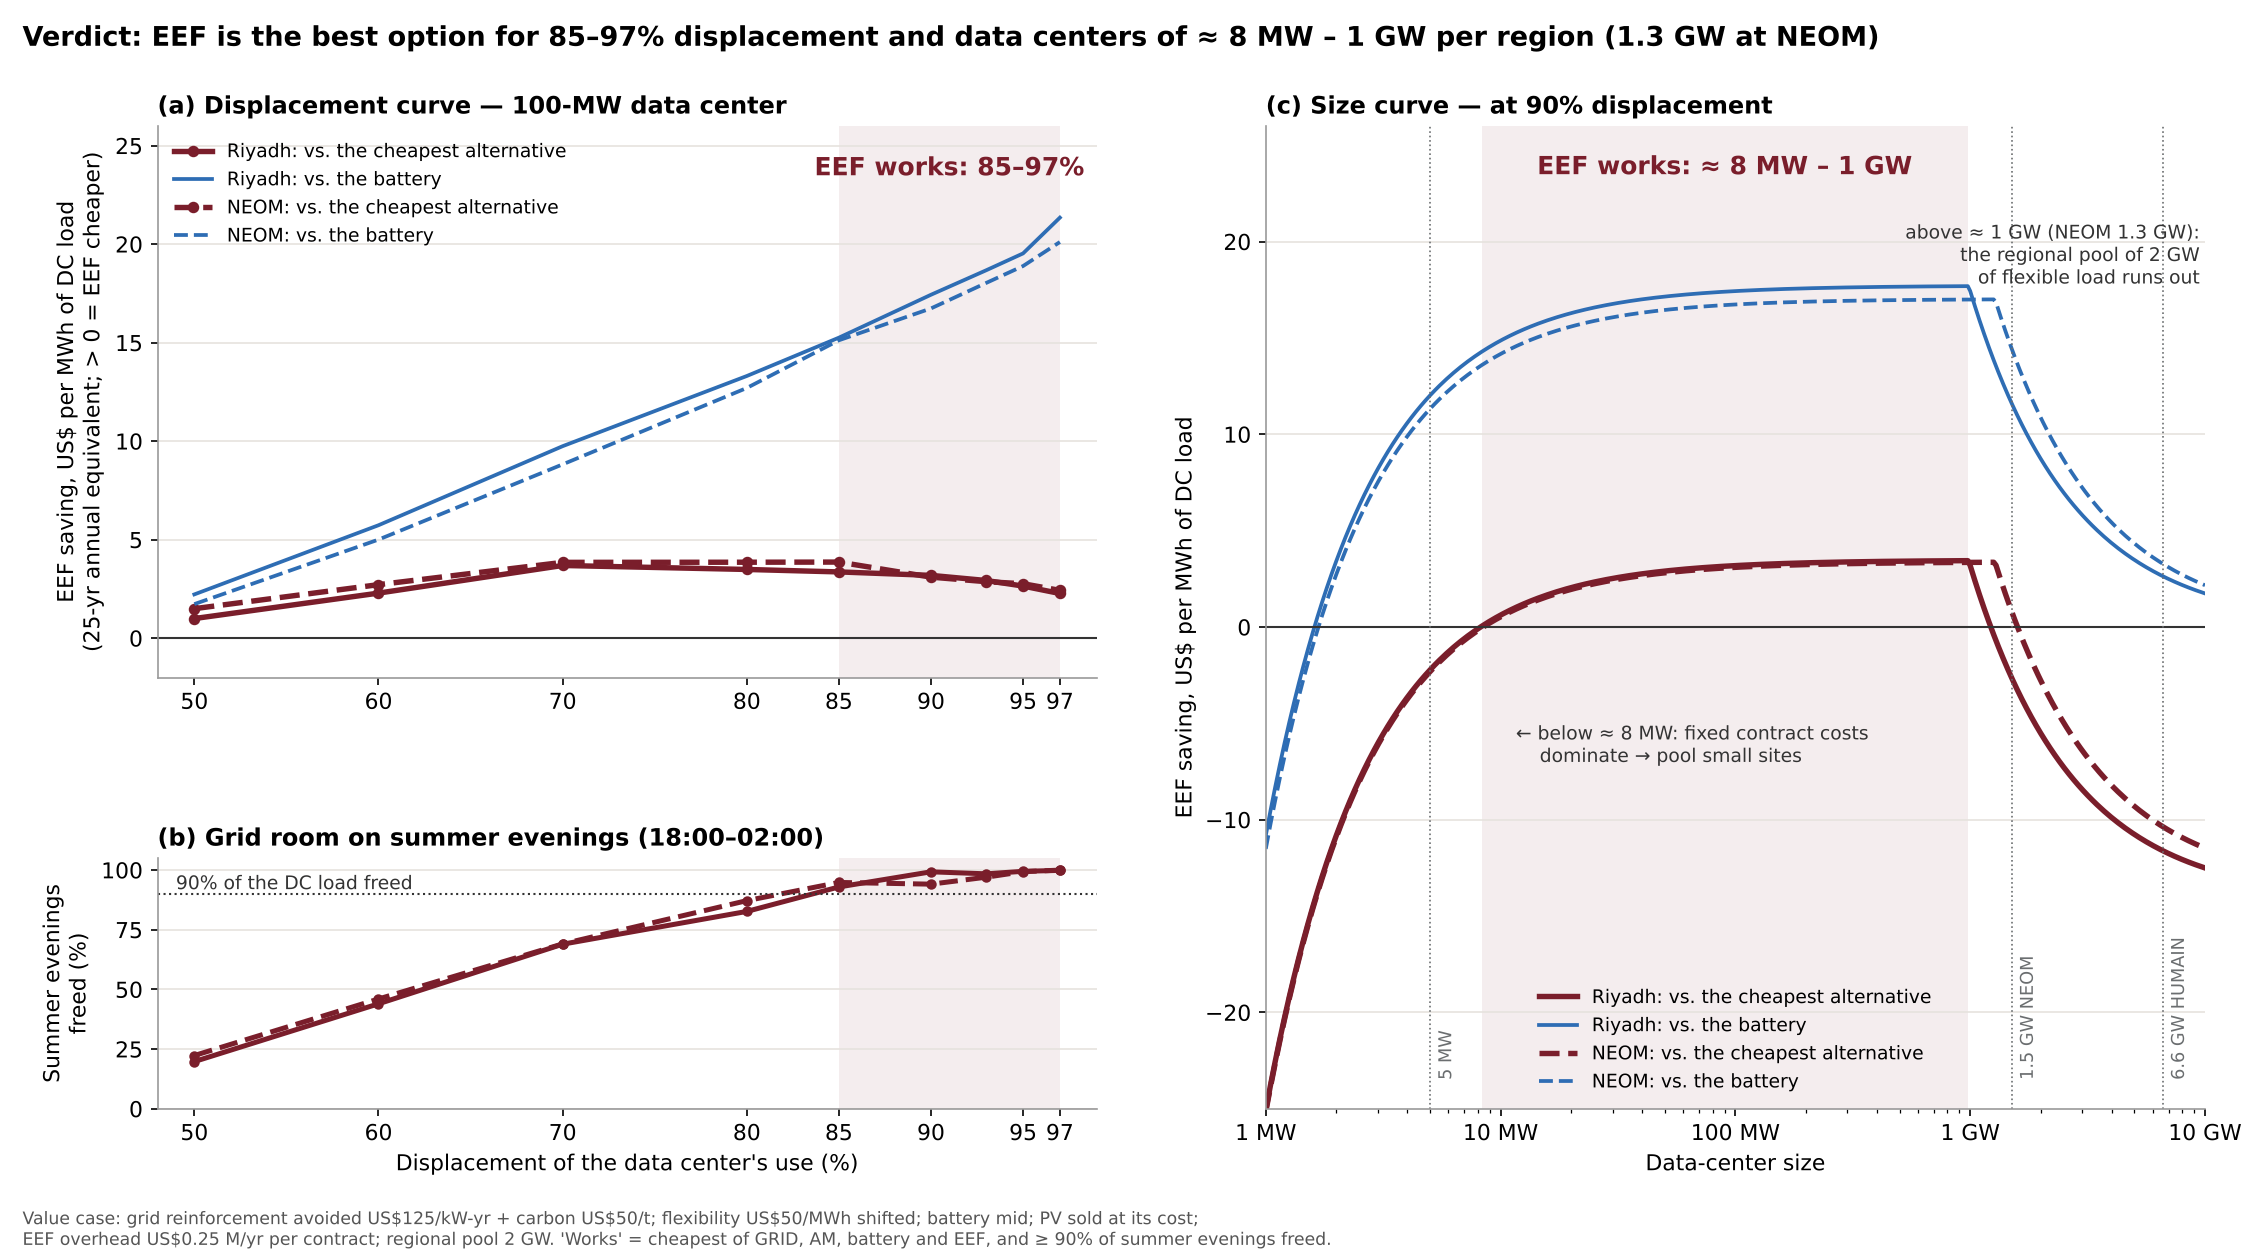
\includegraphics[width=\textwidth]{fig_verdict_curves.png}
\caption{The two curves for Riyadh and NEOM. (a) EEF's saving per MWh against the cheapest alternative and against the battery across displacement targets (100-MW data center); (b) share of summer evenings freed; (c) EEF's saving across data-center sizes at 90\%. Value case: reinforcement US\$125/kW-yr, carbon US\$50/t, flexibility US\$50/MWh shifted, battery mid case, overhead US\$0.25~M/yr.}
\label{fig:3-verdict}
\end{figure}

\section{Results at the 90\% Target}\label{sec:3-8}

\subsection{Flexibility Needed}

Figure~\ref{fig:3-cfe} shows the maximum displacement against contracted flexible power. Displacement rises almost linearly to about 80\% at $P^F/L=1.4$ and saturates at 91.2\% above $P^F/L\approx2.4$. With $D\ge 8$~h, flexible power rather than duration binds: 8 and 12~h give identical results, whereas 4~h needs about 1.5 times the power at 90\% (310 instead of 203~MW). Reaching 60\%, 80\% and 90\% requires 63, 140 and 203~MW of flexibility, or 501, 1,027 and 1,320~MWh of batteries.

\begin{figure}[!htbp]
\centering
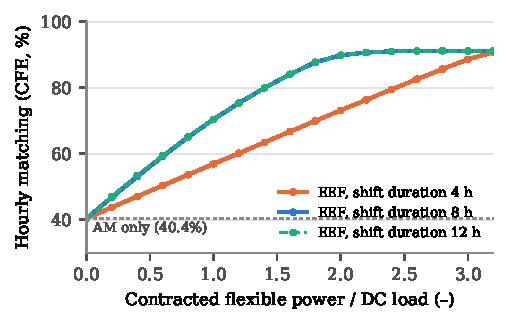
\includegraphics[width=0.75\textwidth]{fig3_cfe_vs_flex.pdf}
\caption{Maximum displacement versus contracted flexible power for three shifting durations (Riyadh, 100~MW).}
\label{fig:3-cfe}
\end{figure}

\subsection{Three Pillars}

Table~\ref{tab:3-pillars} compares the four configurations at 90\%. Grid purchases, US\$42.0~million per year, are identical in all of them.

\begin{table}[!htbp]
\centering
\caption{Three-pillar comparison at 90\% displacement (100-MW data center, Riyadh).}
\label{tab:3-pillars}
\small
\renewcommand{\arraystretch}{1.12}
\begin{tabularx}{\textwidth}{>{\raggedright\arraybackslash}Xcccc}
\toprule
 & \textbf{GRID} & \textbf{AM} & \textbf{RE+BESS} & \textbf{EEF} \\
\midrule
\multicolumn{5}{@{}l}{\emph{Reliability of the data center}} \\
Supply source & Grid & Grid & Grid & Grid \\
Energy not served & 0 & 0 & 0 & 0 \\
If the resource fails & -- & -- & displacement falls & falls to AM \\
\midrule
\multicolumn{5}{@{}l}{\emph{Sustainability}} \\
Displacement (\%) & 0 & 40.4 & 90.0 & 90.0 \\
Emissions (kt CO$_2$/yr) & 498 & 296 & 49.8 & 49.8 \\
New storage (MWh) & 0 & 0 & 1,320 & 0 \\
\midrule
\multicolumn{5}{@{}l}{\emph{Cost}} \\
Matching cost (US\$~M/yr) & 0 & $\approx 0$ & 38.7 (23.2--63.3) & 21.7 (10.9--32.6)$^\ast$ \\
\midrule
\multicolumn{5}{@{}l}{\emph{Impact on the grid}} \\
Load 19:00--23:00 (MW) & 100 & 100 & 6 & 5 \\
Load 00:00--06:00 (MW) & 100 & 100 & 24 & 10 \\
\bottomrule
\multicolumn{5}{@{}p{0.97\textwidth}@{}}{\footnotesize $^\ast$At US\$50 (25--75) per MWh shifted. PV is sold at a price that recovers its cost, so AM adds no net cost. Emissions use the hourly unmatched energy and 0.568~tCO$_2$/MWh. Load: annual average added to the grid by the data center and its resources.}
\end{tabularx}
\end{table}

\emph{Reliability.} The data center is supplied by the grid at all times in every configuration, so its reliability under EEF equals that of direct grid supply. EEF never acts on the data center; if the flexible loads fail to deliver, only displacement falls, at worst to the annual-matching level.

\emph{Sustainability.} EEF and the battery reach the same 90\% and the same emissions, 49.8~kt/yr: a sixth of those under annual matching and a tenth of those under direct grid supply. EEF does so without 1,320~MWh of new batteries.

\emph{Cost.} The battery costs US\$38.7~million per year; EEF costs US\$21.7~million at US\$50/MWh shifted. The break-even price (\ref{eq:3-breakeven}) is US\$89.2/MWh shifted (US\$53--146 across battery cost cases), or US\$191 per kW-yr of contracted power. On the bill alone, without valuing reinforcement or carbon, EEF wins if the single buyer pays about US\$33/MWh for the EEF-linked PV, still below the US\$48/MWh tariff.

\subsection{Seasons, Sensitivities and the Second Site}

Figure~\ref{fig:3-monthly} shows the monthly displacement at an annual target of 90\%. EEF and the battery stay within two points of each other in every month (95.9\% against 96.2\% in June, 77.7\% against 78.7\% in December). Both fall in winter, when PV output is lowest; the battery can carry energy across days, whereas daily windows cannot.

\begin{figure}[!htbp]
\centering
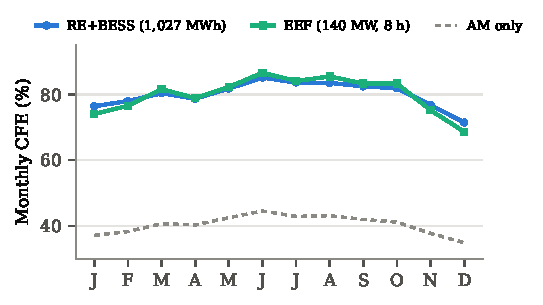
\includegraphics[width=0.75\textwidth]{fig5_monthly.pdf}
\caption{Monthly displacement at a 90\% annual target (Riyadh).}
\label{fig:3-monthly}
\end{figure}

Oversizing PV by 25--50\% raises the base design's ceiling from 91.2\% to 93.1--93.7\% and cuts the flexibility needed for 90\% from 203 to 162--151~MW, while the battery falls only from 1,320 to 1,252--1,227~MWh. A shifting efficiency of 0.85 instead of 0.95 lowers the ceiling to 89.3\% but leaves the break-even price per MWh shifted unchanged. In NEOM, annual matching gives 41.5\% and the base design reaches at most 89.5\%, so 90\% needs PV $\times1.25$ with a window from 09:00. It then needs 157~MW of flexibility or 1,223~MWh of batteries, with a break-even price of US\$86.1/MWh. The concept is not specific to one location.

\section{Scenarios Along the Displacement Curve}\label{sec:3-9}

Table~\ref{tab:3-disp} and Figure~\ref{fig:3-scen}a--c follow a 100-MW data center from 42\% to 100\% displacement. In every row, the data center's load is served in full.

\begin{table}[!htbp]
\centering
\caption{Scenarios along the displacement curve (Riyadh, per 100~MW). Costs above the tariff in US\$/MWh of data-center load (value case); evening load on summer evenings in MW.}
\label{tab:3-disp}
\footnotesize
\setlength{\tabcolsep}{3.5pt}
\renewcommand{\arraystretch}{1.1}
\begin{tabular}{@{}rlccccccccc@{}}
\toprule
& & \textbf{Flex} & \textbf{Battery} & \multicolumn{4}{c}{\textbf{Cost (US\$/MWh)}} & \textbf{Emissions} & \multicolumn{2}{c}{\textbf{Evening load}} \\
\cmidrule(lr){5-8}\cmidrule(lr){10-11}
\textbf{$X$ (\%)} & \textbf{EEF design} & (MW) & (MWh) & GRID & AM & BESS & EEF & (kt/yr) & BESS & EEF \\
\midrule
42 & PV$\times$1.25, 09:00 & 2 & 14 & 42.7 & 31.2 & 31.0 & 31.0 & 289 & 98 & 98 \\
50 & PV$\times$1.25, 09:00 & 28 & 217 & 42.7 & 31.2 & 32.4 & 30.2 & 249 & 77 & 80 \\
60 & PV$\times$1.25, 09:00 & 62 & 472 & 42.7 & 31.2 & 34.7 & 28.9 & 199 & 52 & 56 \\
70 & PV$\times$1.25, 09:00 & 99 & 730 & 42.7 & 31.2 & 37.3 & 27.5 & 149 & 30 & 31 \\
80 & PV$\times$1.25, 09:00 & 137 & 990 & 42.7 & 31.2 & 41.0 & 27.7 & 99.5 & 15 & 17 \\
\textbf{85} & PV$\times$1, 06:00 & 165 & 1,120 & 42.7 & 31.2 & 43.1 & 27.8 & 74.6 & 9.1 & 7.1 \\
\textbf{90} & PV$\times$1, 06:00 & 203 & 1,252 & 42.7 & 31.2 & 45.5 & 28.0 & 49.8 & 4.6 & 0.7 \\
\textbf{95} & PV$\times$1.25, 09:00 & 205 & 1,388 & 42.7 & 31.2 & 48.1 & 28.6 & 24.9 & 1.0 & 0.5 \\
\textbf{98} & PV$\times$1.5, 09:00 & 227 & 1,490 & 42.7 & 31.2 & 50.5 & 28.8 & 10.0 & 0.1 & 0.0 \\
\textbf{99} & PV$\times$3, 09:00 & 206 & 1,459 & 42.7 & 31.2 & 49.2 & 28.0 & 5.0 & 0.0 & 0.0 \\
\textbf{99.5} & PV$\times$2, weekly & 263 & 2,016 & 42.7 & 31.2 & 67.7 & 28.6 & 2.5 & 0.0 & 0.0 \\
100 & \multicolumn{10}{l}{not reachable (ceiling about 99.9\%)} \\
\bottomrule
\multicolumn{11}{@{}p{0.97\textwidth}@{}}{\footnotesize Bold: EEF works (cheapest and $\ge$90\% of summer evenings freed). Battery: its own cheapest allowed design, so it can differ from Table~\ref{tab:3-pillars}. GRID and AM leave 100~MW on summer evenings and emit 498 and 296~kt/yr in every row. Full table: \texttt{results/scenarios\_displacement.csv}.}
\end{tabular}
\end{table}

Three regions appear.
\begin{itemize}
\item \textbf{Below 85\%:} EEF is already the cheapest option from 45\% upward, but it leaves 17--98~MW of a 100-MW data center on the grid on summer evenings. It saves money and emissions but does not yet free the grid where reinforcement is decided.
\item \textbf{From 85\% to 99.5\%:} EEF is the cheapest and frees at least 90\% of the evening load. Its cost stays between US\$27.8 and US\$28.8/MWh, while the battery's rises from US\$43 to US\$68/MWh because each further point needs more storage. Emissions fall from 75 to 2.5~kt/yr.
\item \textbf{At 100\%:} no design reaches it (Section~\ref{sec:3-7}).
\end{itemize}

\section{Scenarios Along the Size Curve}\label{sec:3-10}

Table~\ref{tab:3-size} and Figure~\ref{fig:3-scen}d--f follow the data-center size from 0.1~MW to 6~GW at 90\%. Because the per-MW physics is fixed (Section~\ref{sec:3-7-3}), the scenarios differ only through the contract overhead and the national pool of flexible load. Three pools are tested: unlimited, the high estimate of 29.9~GW and the low estimate of 7.1~GW of industrial demand-response potential by 2030 \cite{r23}. When the pool is short, EEF covers the share $f=\min\{1,\ \text{pool}/(P^F\!\cdot S)\}$ and a battery covers the rest.

\begin{table}[!htbp]
\centering
\caption{Scenarios along the size curve at 90\% (Riyadh). Costs above the tariff in US\$/MWh; evening load on summer evenings.}
\label{tab:3-size}
\footnotesize
\setlength{\tabcolsep}{3.2pt}
\renewcommand{\arraystretch}{1.1}
\begin{tabular}{@{}rcccccccccc@{}}
\toprule
\textbf{Size} & \multicolumn{2}{c}{\textbf{EEF cost}} & \textbf{Cheapest} & \textbf{Flex} & \multicolumn{3}{c}{\textbf{Evening load (MW)}} & \multicolumn{2}{c}{\textbf{Emissions (Mt/yr)}} & \textbf{Reinf. avoided} \\
\cmidrule(lr){2-3}\cmidrule(lr){6-8}\cmidrule(lr){9-10}
(MW) & unlim. & 7.1~GW & (7.1~GW pool) & (GW) & GRID & BESS & EEF & GRID & EEF & (US\$~M/yr) \\
\midrule
1 & 56.3 & 56.3 & AM & 0.002 & 1 & 0.05 & 0.01 & 0.005 & 0.0005 & 0.1 \\
8 & 31.3 & 31.3 & AM & 0.016 & 8 & 0.4 & 0.1 & 0.04 & 0.004 & 1.0 \\
10 & 30.6 & 30.6 & EEF & 0.020 & 10 & 0.5 & 0.1 & 0.05 & 0.005 & 1.2 \\
100 & 28.0 & 28.0 & EEF & 0.20 & 100 & 4.6 & 0.7 & 0.50 & 0.05 & 12.4 \\
1,000 & 27.8 & 27.8 & EEF & 2.0 & 1,000 & 46 & 7.5 & 5.0 & 0.50 & 124 \\
1,500 & 27.8 & 27.8 & EEF & 3.0 & 1,500 & 70 & 11 & 7.5 & 0.75 & 186 \\
3,000 & 27.7 & 27.7 & EEF & 6.1 & 3,000 & 139 & 22.5 & 14.9 & 1.5 & 372 \\
4,500 & 27.7 & 31.7 & AM & 9.1 & 4,500 & 209 & 34 (73) & 22.4 & 2.2 & 558 \\
6,000 & 27.7 & 35.1 & AM & 12.2 & 6,000 & 278 & 45 (142) & 29.9 & 3.0 & 744 \\
\bottomrule
\multicolumn{11}{@{}p{0.97\textwidth}@{}}{\footnotesize GRID US\$42.7, AM US\$31.2 and BESS US\$45.5/MWh at every size. Flex: contracted flexible power with an unlimited pool. Evening load in brackets: with the 7.1-GW pool. AM emits 17.8~Mt/yr at 6~GW. Reinforcement avoided against GRID at US\$125/kW-yr. With the 29.9-GW pool every row equals the unlimited case. Full table: \texttt{results/scenarios\_size.csv}.}
\end{tabular}
\end{table}

\begin{figure}[!htbp]
\centering
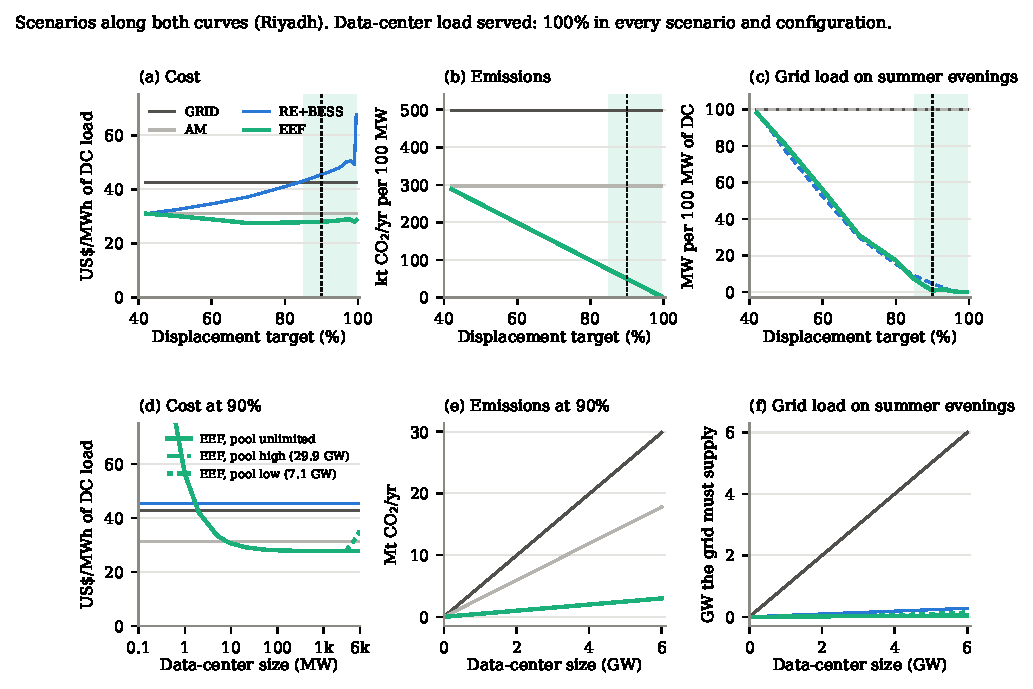
\includegraphics[width=\textwidth]{fig_scenarios.pdf}
\caption{Scenarios along both curves (Riyadh). Top: displacement from 40\% to 100\% for a 100-MW data center: (a) cost above the tariff, (b) emissions, (c) load left on the grid on summer evenings; the shaded band is the range where EEF works. Bottom: size from 0.1~MW to 6~GW at 90\%: (d) cost, with three flexible-load pools, (e) emissions, (f) load left on the grid on summer evenings. The data center's load is served in full in every scenario.}
\label{fig:3-scen}
\end{figure}

The size scenarios show four things.
\begin{enumerate}
\item \textbf{Small sites} (below about 8~MW) pay too much contract overhead per MWh; AM is cheaper, and grouping sites in one contract is the remedy.
\item \textbf{From about 8~MW to 3.5~GW}, EEF is the cheapest with every pool. At 3.5~GW it needs 7.1~GW of flexible load (2.03~MW per MW), the whole low-estimate pool.
\item \textbf{Above 3.5~GW with the low pool}, a battery must cover the rest of the target. The hybrid costs more than AM (US\$31.7 and US\$35.1 against US\$31.2/MWh at 4.5 and 6~GW), but it still leaves only 73--142~MW of a 4.5--6~GW center on the grid on summer evenings. With the high pool, EEF stays the cheapest up to 6~GW and beyond, to about 14.7~GW.
\item \textbf{The grid effect grows with size.} At 6~GW, GRID and AM leave 6,000~MW on the grid on summer evenings, the battery 278~MW and EEF 45~MW. EEF avoids about US\$744~million per year of reinforcement against GRID and cuts emissions from 29.9 to 3.0~Mt/yr.
\end{enumerate}

\section{The National Grid Context}\label{sec:3-11}

The size scenarios matter because the Saudi grid already has its own growth to serve before any data center connects (Figure~\ref{fig:3-grid} and Table~\ref{tab:3-grid}).

\subsection{Capacity, Peak and Margin}

Installed generation capacity is about 90~GW \cite{v2030cap}. The summer peak, observed by SERA, was 62.3~GW in 2020, 65.3~GW in 2022, 70.7~GW in 2023 and 74.8~GW in 2024 \cite{r23}, and it reached a record 77.1~GW in 2025, 3\% above 2024 \cite{mees2026}. The peak has therefore grown by 14.8~GW in five years, about 3~GW a year. It grows faster than annual consumption (by 8.2\% in 2022--23, against annual demand growth above 2\% since 2020), which KAPSARC attributes to short, intense and temperature-sensitive uses \cite{r23}, and the observed peak has exceeded the 2025 forecast made in 2021 (69.2~GW) every year since 2023 \cite{r23}. The nominal margin between capacity and peak is therefore about 13~GW. Less than that is available on a hot summer evening, when thermal units derate and some are on maintenance, and when PV is no longer generating.

\subsection{New Load Beyond Data Centers}

That margin is shared by all new load: giga-projects, industry, mining, desalination and cooling for a growing population all add to the evening peak. KAPSARC reports that when Ramadan falls in summer, evening and night consumption and continued cooling demand raise the peak further \cite{r23}. The system is expanding to meet this growth. By 2030, variable renewable capacity is to rise from 4.1~GW (2024) to 100--130~GW, supported by about 110~GW of gas capacity, 48~GWh of batteries and interconnection rising from 1.6 to 7.4~GW \cite{r23}. That expansion, however, is sized for the load already expected; and renewables do not generate on summer evenings. KAPSARC also estimates all Saudi data centers at 10~TWh/yr in 2030 in a business-as-usual case and 20~TWh/yr with moderate AI growth \cite{r23}, a constant load of 1.1--2.3~GW.

\subsection{What a Data Center Adds}

Table~\ref{tab:3-grid} expresses the evening load of each configuration in national terms. A 1.5-GW center supplied by the grid alone adds 1.9\% of the 2025 peak; a 6-GW center adds 7.8\%, uses 46\% of the nominal margin and equals two years of national peak growth. With EEF, the same 6-GW center adds 45~MW, or 0.06\% of the peak, because the freed supply comes from loads that already exist.

\begin{table}[!htbp]
\centering
\caption{Load left on the grid on summer evenings at 90\%, against the national peak (77.1~GW in 2025), the nominal margin (12.9~GW) and one year of peak growth (3.0~GW).}
\label{tab:3-grid}
\small
\renewcommand{\arraystretch}{1.15}
\begin{tabular}{@{}rccccc@{}}
\toprule
\textbf{Data center} & \multicolumn{3}{c}{\textbf{Evening load (MW)}} & \multicolumn{2}{c}{\textbf{GRID as a share of}} \\
\cmidrule(lr){2-4}\cmidrule(lr){5-6}
\textbf{(GW)} & \textbf{GRID} & \textbf{RE+BESS} & \textbf{EEF} & \textbf{peak} & \textbf{margin} \\
\midrule
0.1 & 100 & 4.6 & 0.7 & 0.13\% & 0.8\% \\
1.0 & 1,000 & 46 & 7.5 & 1.3\% & 7.7\% \\
1.5 & 1,500 & 70 & 11 & 1.9\% & 11.6\% \\
3.0 & 3,000 & 139 & 22.5 & 3.9\% & 23.2\% \\
6.0 & 6,000 & 278 & 45 & 7.8\% & 46.4\% \\
\bottomrule
\multicolumn{6}{@{}p{0.8\textwidth}@{}}{\footnotesize EEF at 6~GW: 0.06\% of the peak and 0.35\% of the margin (142~MW with the 7.1-GW pool). Full table: \texttt{results/grid\_context\_dc.csv}; sources: \texttt{results/saudi\_grid\_context.csv}.}
\end{tabular}
\end{table}

\begin{figure}[!htbp]
\centering
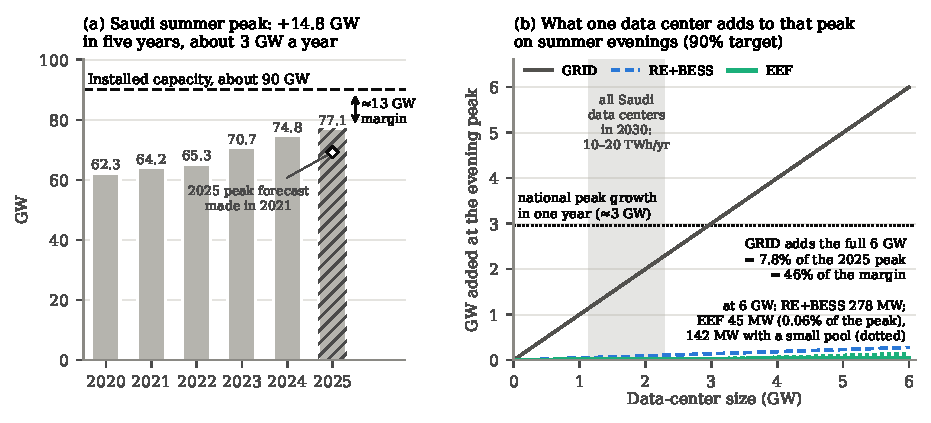
\includegraphics[width=\textwidth]{fig_grid_context.pdf}
\caption{(a) Saudi summer peak, 2020--2025, against installed capacity of about 90~GW; the hatched bar (2025) is from \cite{mees2026}, the others from SERA data in \cite{r23}; the diamond is the 2025 forecast made in 2021. (b) Load a data center adds to the summer-evening peak at 90\%, by configuration; the band marks all Saudi data centers in 2030 (10--20~TWh/yr), and the dotted line one year of national peak growth.}
\label{fig:3-grid}
\end{figure}

\subsection{The Texas Lesson}

Texas shows what happens when large constant loads arrive faster than the grid can be expanded. ERCOT's large-load interconnection queue grew from more than 233~GW at the end of 2025 to about 474~GW by mid-2026, about 90\% of it data centers \cite{utilitydive2026,ercot2026}, and only 22~GW had met ERCOT's study requirements by April 2026 \cite{ercot2026}. Texas Senate Bill~6 (June 2025) now lets transmission providers curtail non-critical new large loads in grid emergencies and adds interconnection standards and batch studies \cite{sidley2025}. Expansion of generation, transmission and substations then becomes the bottleneck, with long lead times and costs borne by all customers. These queue figures differ across sources and dates and are not forecasts of what will be built.

EEF offers Saudi Arabia a different path. A data center under EEF is fully grid-connected, so it keeps grid-level reliability, yet at 90\% it adds almost nothing to the summer-evening peak and leaves only 10~MW of every 100~MW on the grid between midnight and 06:00 (24~MW with a battery; Table~\ref{tab:3-pillars}). The system can therefore host large data centers within its existing generation and much of its shared network, and keep the margin for the growth it already expects. Two cautions apply. The data center's own connection must still be sized for its full load, so the relief is at system level, upstream of its substation, not at the substation itself. And because flexible loads may sit in other regions, the transfer capacity between regions must be checked (Chapter~6).

\section{Code and Reproducibility}\label{sec:3-12}

All results in this chapter come from Python~3 scripts in \texttt{tpec2027/model/}, using NumPy, SciPy (HiGHS) and Matplotlib. Table~\ref{tab:3-code} lists them in the order they run. Every number in the chapter is written to a CSV file in \texttt{tpec2027/results/}, so each can be traced to the script that produced it.

\begin{table}[!htbp]
\centering
\caption{Code used in this chapter (\texttt{tpec2027/model/}).}
\label{tab:3-code}
\small
\renewcommand{\arraystretch}{1.15}
\begin{tabularx}{\textwidth}{>{\raggedright\arraybackslash}p{4.1cm}>{\raggedright\arraybackslash}X>{\raggedright\arraybackslash}p{4.1cm}}
\toprule
\textbf{Script} & \textbf{What it does} & \textbf{Output} \\
\midrule
\texttt{eef\_model.py} & Data, profiles and the linear programs: EEF min-capacity (\ref{eq:3-min}) and max-displacement (\ref{eq:3-max}), battery min-energy, battery annual cost & used by all scripts \\
\texttt{run\_experiments.py},\newline \texttt{run\_extra.py} & Annual-matching baseline, displacement versus flexible power, targets, sensitivities & \texttt{baseline}, \texttt{cfe\_vs\_flex},\newline \texttt{targets}, \texttt{sens\_*} \\
\texttt{run\_ceiling.py} & Why EEF stops short of 100\% & \texttt{ceiling} \\
\texttt{run\_displacement.py} & The sweep: targets $\times$ designs (66 LPs for Riyadh, 70 for NEOM) & \texttt{displacement\_curve*} \\
\texttt{plot\_displacement.py} & Cost model (\ref{eq:3-unitcost}), design choice, value cases & \texttt{displacement\_costs} \\
\texttt{plot\_verdict.py} & The two curves and the working ranges & \texttt{verdict\_ranges},\newline Fig.~\ref{fig:3-verdict} \\
\texttt{run\_base.py} & Results at 90\%: pillars, months, sites & \texttt{base\_*} \\
\texttt{check\_scaling.py} & Linear-scaling check & \texttt{scaling\_check},\newline Table~\ref{tab:3-scaling} \\
\texttt{run\_scenarios.py} & Scenarios along both curves & \texttt{scenarios\_*},\newline Fig.~\ref{fig:3-scen} \\
\texttt{grid\_context.py} & National grid context & \texttt{grid\_context\_dc},\newline \texttt{saudi\_grid\_context},\newline Fig.~\ref{fig:3-grid} \\
\bottomrule
\end{tabularx}
\end{table}

\section{Limitations}\label{sec:3-13}

\begin{itemize}
\item \textbf{One flexible class, perfect foresight, one weather year.} The portfolio is one aggregated class, and operation is planned with perfect knowledge of 2020 PV output. Heterogeneous loads and forecast errors are the subject of Chapter~4.
\item \textbf{Assumed prices.} Flexibility costs are unknown in Saudi Arabia, so the results are given as break-even values and ranges. The reinforcement and carbon values and the contract overhead are assumptions, tested over ranges.
\item \textbf{Battery cost.} Only energy capacity is charged, which favors storage.
\item \textbf{Emissions at the average factor.} In Saudi Arabia the marginal generator often changes little with load timing \cite{r38}, so the benefit of shifting depends on midday PV that would otherwise be curtailed, which becomes more frequent as solar penetration rises \cite{r23,r44}.
\item \textbf{Single node.} Network constraints and transfers between regions are not modeled; the flexible-load potential was estimated for peak shaving rather than daily shifting \cite{r23}; and baselines can be gamed \cite{r45}. These are tested in Chapter~6.
\item \textbf{National figures.} The 2025 peak is taken from a trade publication \cite{mees2026} and the installed capacity from a secondary source \cite{v2030cap}; both should be checked against SERA's annual statistics.
\item \textbf{Design set.} The sweep uses a window from 06:00 with PV equal to the annual use, and from 09:00 with larger plants. A window from 09:00 with PV equal to the annual use reaches 93.4\% and may lower the flexible power needed at 90\%; it is a refinement for Chapter~5.
\end{itemize}

\section{Summary}\label{sec:3-14}

This chapter defined External Energy Flexibility, formulated it as linear programs solved with HiGHS, and compared it with grid supply, annual matching and batteries. Instead of assuming a target or a size, it swept both, and the results answer the first research question.
\begin{itemize}
\item EEF keeps the data center's reliability equal to the grid's, because the data center never leaves the grid.
\item EEF works for displacement targets of 85--99.5\% and data centers from about 8~MW; 90\% is the recommended target.
\item At 90\%, EEF matches the battery's emissions, a sixth of those under annual matching, with 203~MW of contracted flexibility instead of 1,320~MWh of batteries, and is cheaper whenever flexibility costs less than about US\$89 per MWh shifted.
\item Per MW, the physics does not depend on size; size matters through the contract overhead at the small end and through the national pool of flexible load at the large end (3.5~GW with the low estimate, about 14.7~GW with the high one).
\item On a grid of about 90~GW whose peak grows by about 3~GW a year, a 6-GW data center on grid supply alone would take 46\% of the nominal margin on summer evenings; under EEF it takes 0.35\%.
\end{itemize}
EEF thus lets Saudi Arabia host large AI data centers with high reliability, at the lowest cost and with the lowest emissions, without forcing the grid into the rushed expansion seen in Texas. Chapter~4 turns to operating EEF under uncertainty.


\begin{singlespace}
\bibliographystyle{IEEEtran}
\bibliography{refs,../../tpec2027/paper/refs_extra,refs_ch3}
\end{singlespace}
\end{document}
